\chapter{Gravwell Kits}
\label{ch:kits}
\index{Kits}
Gravwell Kits act like a sort of `app store' from which Gravwell users can
install kits to gain out-of-box capabilities for common technologies. As
an example, let's take an organization that uses Zeek for firewall/IDS
logging on their network. These logs are ingested by Gravwell and easily
searchable, but the users must issue their own queries to explore and
analyze that data. This requires knowledge and experience with both
Gravwell and Zeek in order to create useful dashboards, automation,
data enrichments, or otherwise get value out of the data using Gravwell.

With Gravwell Kits, that organization can install the pre-built and
signed kit for Zeek. This comes with:

\begin{itemize}
\tightlist
\item
  Commonly-used dashboards for quick situational awareness and heads-up
  monitoring of Zeek activity.
\item
  Scheduled searches which look for statistical anomalies within the
  Zeek data and alert when any are discovered.
\item
  Investigative dashboards that search Zeek data for items of interest
  such as IP addresses found in other logs or data within Gravwell.
\item
  Search Templates for easily running common queries.
\item
  Threat intelligence resources that search Zeek events for
  known-malicious activity.
\item
  And more!
\end{itemize}

Creating Gravwell kits isn't very different than the hands-on activity we
have been conducting to date. Building dashboards, setting up automated
searches, loading data enrichment resources--all of these things are
what goes into developing a cohesive kit. These Gravwell resources are
bundled up, digitally signed, and distributed via Gravwell infrastructure
to users. Because these kits can include Gravwell scripts (which are
Turing-complete programs), the Gravwell team assesses and digitally
signs all kits approved for distribution.

This chapter shows how to browse, install, and explore kits. It also
discusses the kit building process, which allows you to package things
you build to share with friends and colleagues.

The `Kits' section of the Gravwell web UI is the centralized place to work with kits. You can find the Kits page in the main menu, as shown in Figure \ref{fig:kit-menu}.

\begin{figure}
	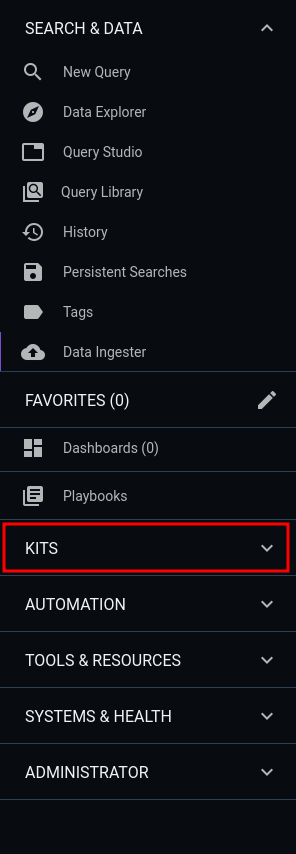
\includegraphics[width=0.3\linewidth]{images/kit-menu.png}
	\caption{Kits menu item}
	\label{fig:kit-menu}
\end{figure}

\section{What's in a Kit?}

There are many components which make up a kit. First, there are the contents of the kit, which fall into 2 categories:

\begin{itemize}
\tightlist
\item
  Items: Regular Gravwell components such as dashboards, scheduled searches, macros, actionables, etc.
\item
  Configuration Macros: These are specialized macros which the kit uses to configure itself, which can allow greater flexibility in e.g. choices of tags used. For instance, rather than using tag=netflow in all queries, a Netflow kit can say \code{tag=\$NETFLOW\_KIT\_TAG}, then define a configuration macro named \code{NETFLOW\_KIT\_TAG}. At installation time, the kit prompts the user for which tag or tags contain Netflow records.
\end{itemize}

There are a few other things which help identify a kit that are useful to keep in mind:

\begin{itemize}
\tightlist
\item
ID: Identifies the kit. Gravwell uses namespaces similar to Android applications, e.g. "io.gravwell.netflow".
\item
Version: Kits may be updated over time, and the version number tracks this so Gravwell can automatically notify of new kit versions.
\item
Name: A user-friendly name for the kit, e.g. "Netflow v5".
\item
Description: A detailed description of what the kit does.
\item
MinVersion/MaxVersion: Some kits require specific Gravwell features; to ensure those features are available, these fields specify which Gravwell versions are compatible with the kit.
\item
Dependencies: Kits can depend on other kits, like packages in a Linux distribution. Gravwell's Netflow v5 kit depends on the Network Enrichment kit, for example. Dependencies are automatically installed along with the kit.
\end{itemize}

\subsection{Dependencies}
\index{Kits!dependencies}:
A kit may have \emph{dependencies} defined. Dependencies are other kits which the kit requires for proper functionality. For example, many kits depend on the Network Enrichment kit, which provides some baseline resources for enriching network data, such as a GeoIP database. Dependencies are installed automatically when you deploy a kit, provided the dependency exists on the Gravwell kit server.

\section{Browsing and Installing Kits}
\index{Kits!installation}
On a fresh Gravwell cluster, no kits are installed. Opening the `Kits' section will present an empty page (Figure \ref{fig:blank-kits}). If you click `Manage Kits', you will be taken directly to the list of kits on the Gravwell kit server, as shown in Figure \ref{fig:available-kits}.

\begin{figure}
	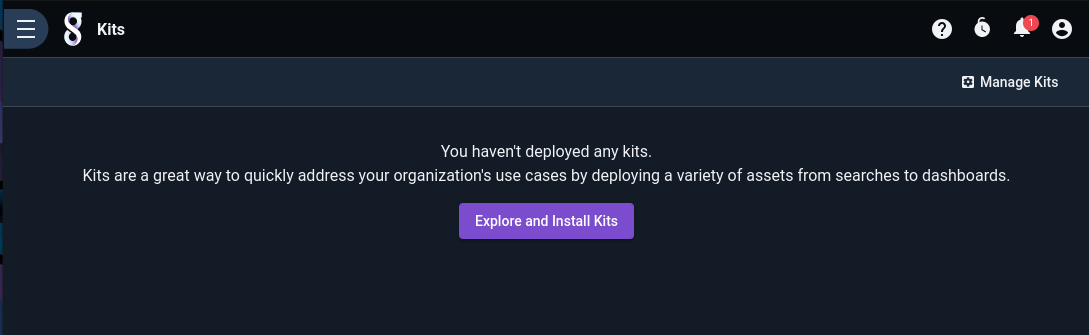
\includegraphics[width=0.85\linewidth]{images/blank-kits.png}
	\caption{Kits page on a new Gravwell installation}
	\label{fig:blank-kits}
\end{figure}

\begin{figure}
	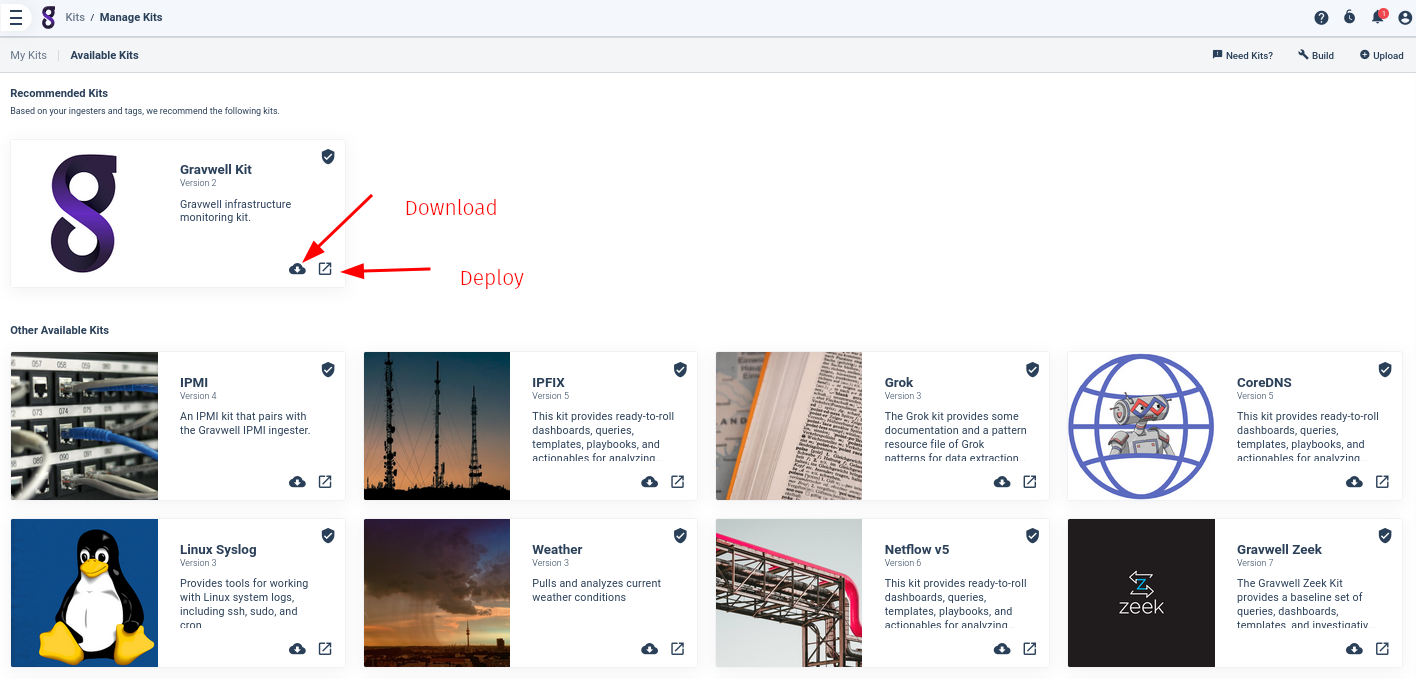
\includegraphics[width=0.85\linewidth]{images/available-kits.png}
	\caption{Browsing available kits}
	\label{fig:available-kits}
\end{figure}

You can click the kit details button to learn more about a given kit. Once you've decided on a kit to install, click the install kit button. The system will download the kit, then pop up a wizard for installation. In Figure \ref{fig:wizard1}, we have selected the IPFIX kit for installation. The first page shows a list of items contained in the kit; after reviewing the contents, click the checkbox and select the Next button. The wizard will then display any licenses packaged with the kit, as seen in Figure \ref{fig:wizard2}. Note that if there are multiple licenses, you will have to select each one individually from the list on the left and click each checkbox before continuing.

\begin{figure}
	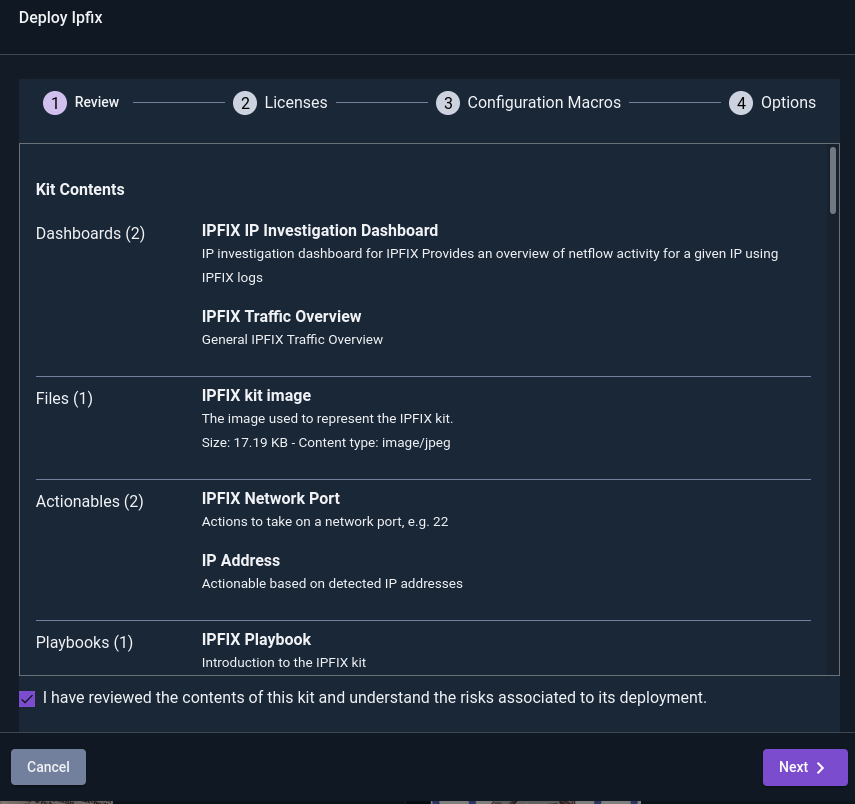
\includegraphics[width=0.6\linewidth]{images/wizard1.png}
	\caption{Installing IPFIX kit, step 1}
	\label{fig:wizard1}
\end{figure}

\begin{figure}
	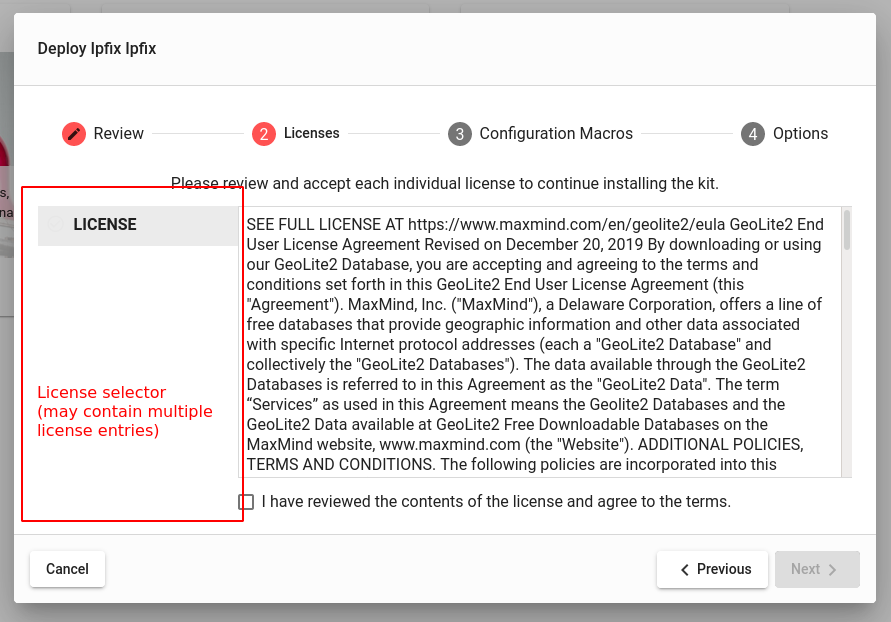
\includegraphics[width=0.6\linewidth]{images/wizard2.png}
	\caption{Installing IPFIX kit, step 2}
	\label{fig:wizard2}
\end{figure}

Next, the wizard will prompt for Configuration Macros, if any are defined by the kit. Figure \ref{fig:wizard3} shows this step. A configuration macro allows install-time configuration of the queries which are shipped by the kit; these will typically include a default value but also provide a description to help you figure out what to enter. In the screenshot, it needs to know which tag contains IPFIX records; because we intend to use the \code{ipfix} tag, we can leave the default value alone.

\begin{figure}
	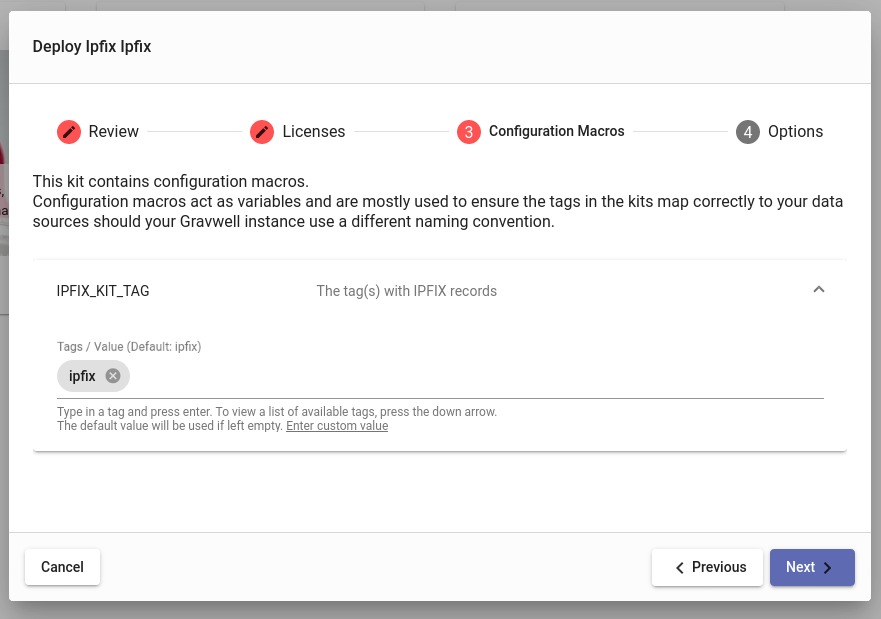
\includegraphics[width=0.6\linewidth]{images/wizard3.png}
	\caption{Installing IPFIX kit, step 3}
	\label{fig:wizard3}
\end{figure}

The final page of the wizard (Figure \ref{fig:wizard4} prompts for additional options. ``Override Existing Items'', if checked, will overwrite any conflicting objects which may already exist on the system--for instance, if you have created a resource named ``foo'', but the kit will also create a resource named ``foo''. The ``Group Access'' dropdown allows you to optionally select a group which can see the contents of the kit. Admin users will also have the option to install the kit globally, meaning all users can see it.

\begin{figure}
	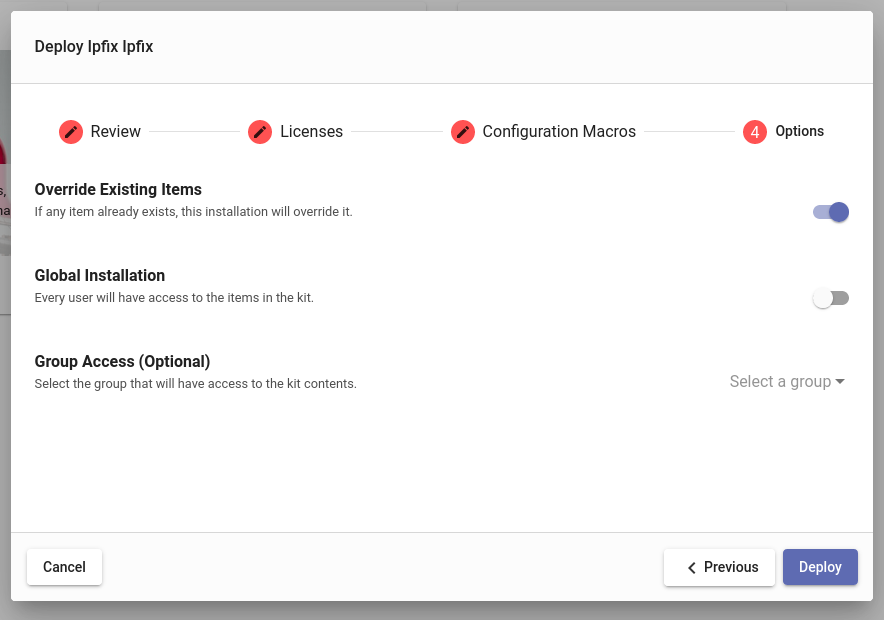
\includegraphics[width=0.6\linewidth]{images/wizard4.png}
	\caption{Installing IPFIX kit, step 4}
	\label{fig:wizard4}
\end{figure}

When you click the ``Deploy'' button, the kit and any dependencies will be installed. The GUI will display kit installation status as it goes. It may take some time, but eventually the installation will complete as shown in Figure \ref{fig:install-done}.

\begin{figure}
	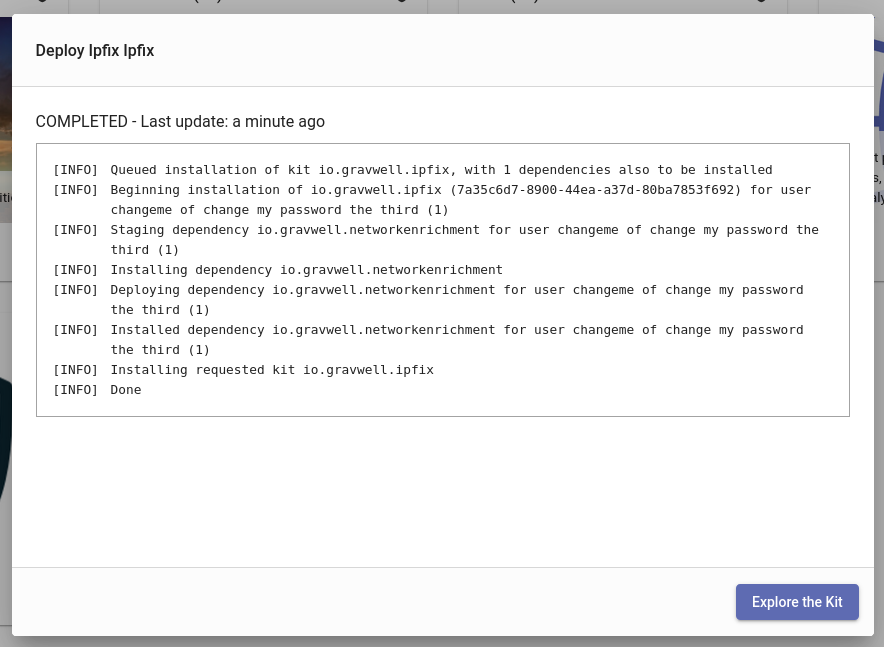
\includegraphics[width=0.6\linewidth]{images/install-done.png}
	\caption{Kit deployment status}
	\label{fig:install-done}
\end{figure}

\clearpage

\subsection{Exploring a Kit}

If you click `Explore the Kit' on the kit installation dialog (Figure \ref{fig:install-done}, you'll be taken to a page outlining the contents of the kit, as seen in Figure \ref{fig:explore}.

\begin{figure}[H]
	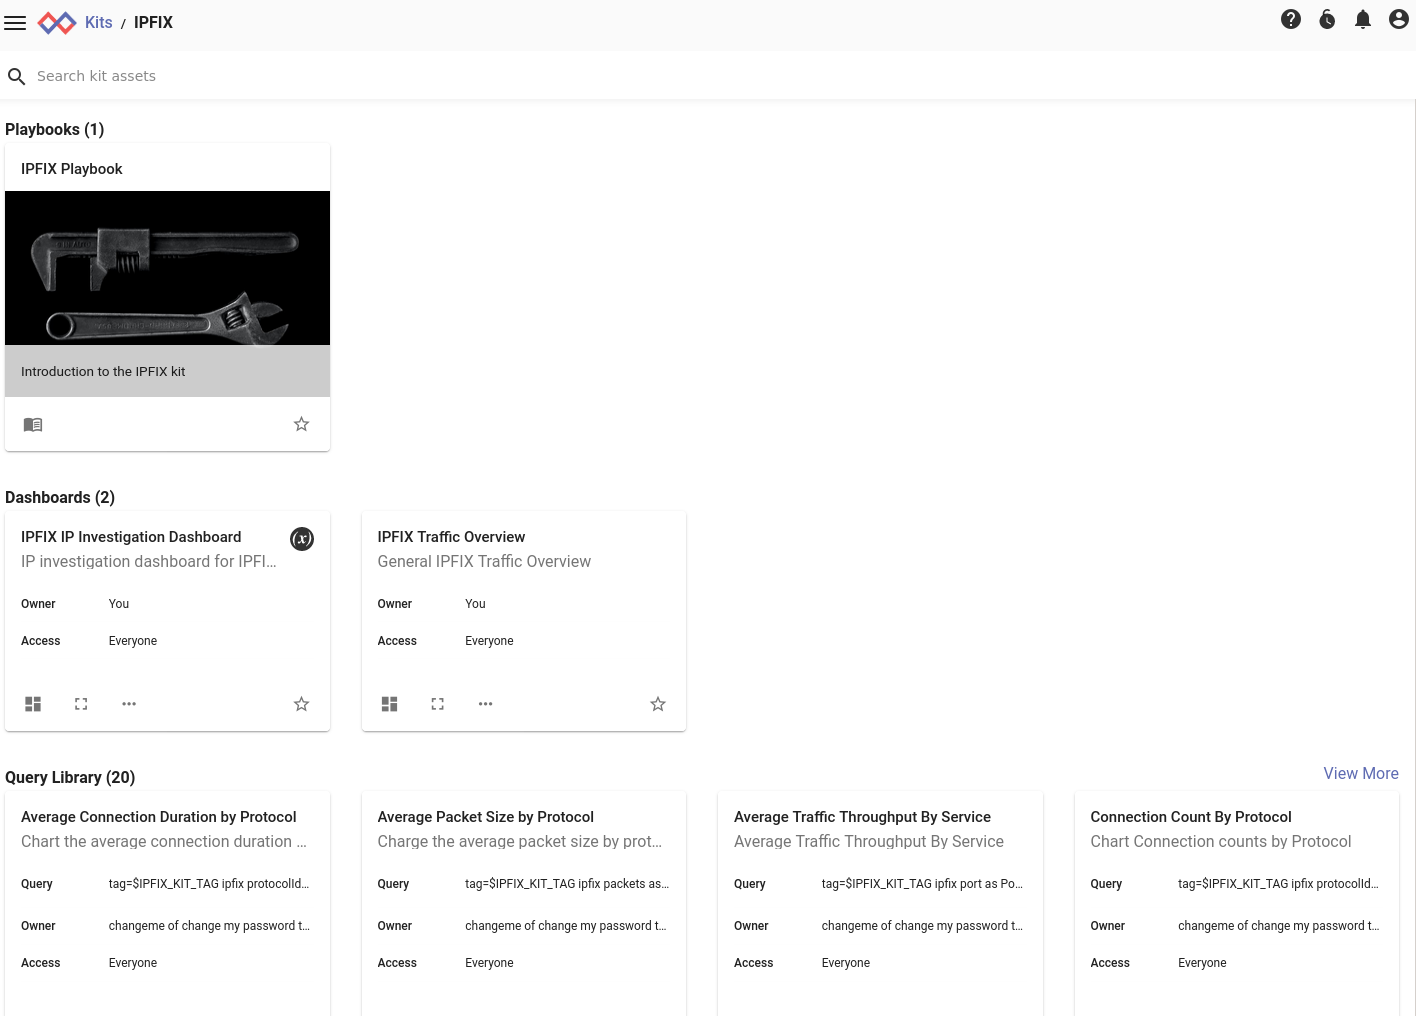
\includegraphics[width=0.8\linewidth]{images/explore.png}
	\caption{Exploring a kit}
	\label{fig:explore}
\end{figure}

 Note that opening the kit like this (or clicking its icon in the list of installed kits) puts you in the kit's \emph{context}. You can tell you are inside a kit context because the text ``Kits / IPFIX'' is in the top bar of the UI. While you're in a kit context, the UI will only show items contained within the kit. To leave the kit context, either click the Gravwell logo at the top of the page, or click `Exit kit' in the main menu.

You can always re-visit an installed kit by opening the kit menu and clicking the kit's icon in the list of installed kits.

\section{Managing Installed Kits}

\subsection{Upgrading Kits}
\index{Kits!upgrading}
Once a kit has been installed, little administration is required. The sole point of manual intervention required is \emph{upgrading} a kit when a new version comes out. Gravwell will periodically push updates to the official kit server. When one of your installed kits has an update available, an ``Upgrade'' button will appear on that kit's tile, as shown in Figure \ref{fig:upgradekit}

\begin{figure}[H]
	
\includegraphics[width=0.4\linewidth]{images/upgradekit.png}
	\caption{The kit upgrade notification}
	\label{fig:upgradekit}
\end{figure}

Clicking the button will launch an upgrade wizard similar to the installation wizard. The most important difference is the Backup option. If you have modified any of the items which were included in the kit, the wizard will notify you and provide options for copying or downloading the modified items. If there are no items which have been modified, the Backup step will not be shown. The rest of the wizard is identical to the installation wizard, although defaults such as group access should be already set for you.

Be warned that upgrading a kit to a new version involves the complete deletion of the previous version's contents. Do not click the ``Deploy'' button at the end of the wizard until you are prepared for this to happen!

\subsection{Uninstalling Kits}
\index{Kits!uninstalling}
To remove an installed kit, enter kit management mode by clicking the ``Manage Kits'' button in the upper-right corner of the main kits page. Then select the trash can icon on the desired kit. A dialog will pop up for confirmation, as shown in Figure \ref{fig:uninstall-confirm}. If you then click ``Uninstall'', the kit will be removed, \emph{unless} you have manually changed any of the kit contents. If you have modified any of the kit items, you will see a second dialog warning you of this fact and allowing one last chance to abort the process, as seen in Figure \ref{fig:uninstall-warn}

\begin{figure}[H]
	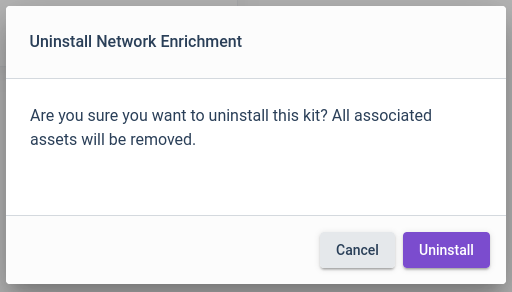
\includegraphics[width=0.4\linewidth]{images/uninstall-confirm.png}
	\caption{Kit deletion dialog}
	\label{fig:uninstall-confirm}
\end{figure}

\begin{figure}[H]
	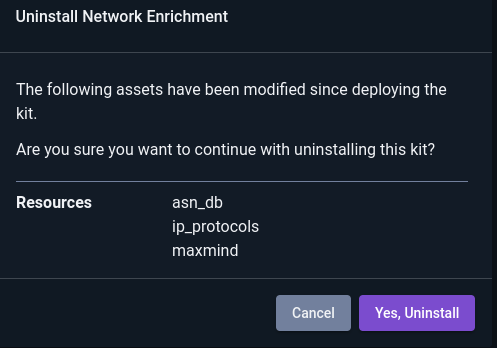
\includegraphics[width=0.4\linewidth]{images/uninstall-warn.png}
	\caption{Kit deletion warning dialog for modified items}
	\label{fig:uninstall-warn}
\end{figure}

\section{Hands-on Lab: Installing Kits}

For this hands on lab we are going to install the Netflow kit, browse some of the kit contents, then uninstall the kit.

Start by cleaning your environment and starting up a new base Gravwell
instance:

\begin{Verbatim}[breaklines=true]
docker stop $(docker ps -q)
docker rm $(docker ps -q -a)
docker create --rm --net gravnet -p 8080:80 --name kits gravwell:base
docker start kits
\end{Verbatim}

Next, start the ingester container running the netflow ingester:

\begin{Verbatim}[breaklines=true]
docker run --rm --net gravnet --name ingesters -it \
-e GRAVWELL_CLEARTEXT_TARGETS=kits:4023 \
gravwell:netflow /opt/gravwell/bin/gravwell_netflow_capture
\end{Verbatim}

The netflow ingester is pre-configured to listen on port 2055 for
incoming Netflow v5 records.

Now, we use another Docker container to generate Netflow records and
send them to the ingester:

\begin{Verbatim}[breaklines=true]
docker run -it --net gravnet --rm \
networkstatic/nflow-generator -t ingesters -p 2055
\end{Verbatim}

The netflow generator will run indefinitely, generating flow records,
until killed.

Log into your Gravwell GUI (\href{http://localhost:8080}{http://localhost:8080}) and navigate to the Kits page. Click `Manage kits', which should take you to the list of available kits. Find and click the deploy button on the Netflow v5 kit, then walk through the installation wizard.

When installation is done, click the `Explore the kit' button, then open the playbook and run some of the sample queries on the Netflow data we're ingesting. Explore the rest of the kit, then try to answer these questions:

\begin{enumerate}
\item
	How many dashboards are included in the kit?
\item
	Click the Gravwell icon at the top of the page to leave the kit context. How do you now get back into the kit contents list?
\item
	Open the Netflow V5 Traffic Overview dashboard, scroll down to the 'Rare Ports' tile, and click one of the IP addresses. If you wanted to add to the actionables, how would you find the actionable definitions?
\end{enumerate}

When you're done, return to the `Manage kits' page and uninstall the kit. Verify that none of the Netflow dashboards or other objects still exist. Note that there is still a kit installed--which kit is it, and why was it installed?

To clean up after the experiment, simply run:

\begin{Verbatim}[breaklines=true]
docker kill $(docker ps -a -q)
\end{Verbatim}

\section{Building Kits}
\index{Kits!building}
Although Gravwell distributes pre-built official kits, any user can build a kit themselves. This is a convenient way to share objects built on one Gravwell instance with another instance. Note that kits built like this are not signed by Gravwell and therefore can only be installed by administrators.

You can build a kit by clicking the `Build' button on the Manage Kits page. This launches the kit-building wizard. On the first page, seen in Figure \ref{fig:buildwizard1}, you set general options. The name should be a user-friendly short name like ``Network Enrichment'', ``Zeek Kit'', etc. The kit ID should be a namespaced and unique ID for your kit; although the field is free-form, we recommend using domain namespaces, e.g. ``io.gravwell.example''. The Version field sets a version for the kit, which is useful for upgrades if you decide to set up your own kit server. The optional Gravwell minimum and maximum versions allow you to restrict the kit's compatiblity to particular versions of Gravwell. Finally, the kit icon field lets you optionally set a small image which may be used by Gravwell to help identify the kit to users.

\begin{figure}[H]
	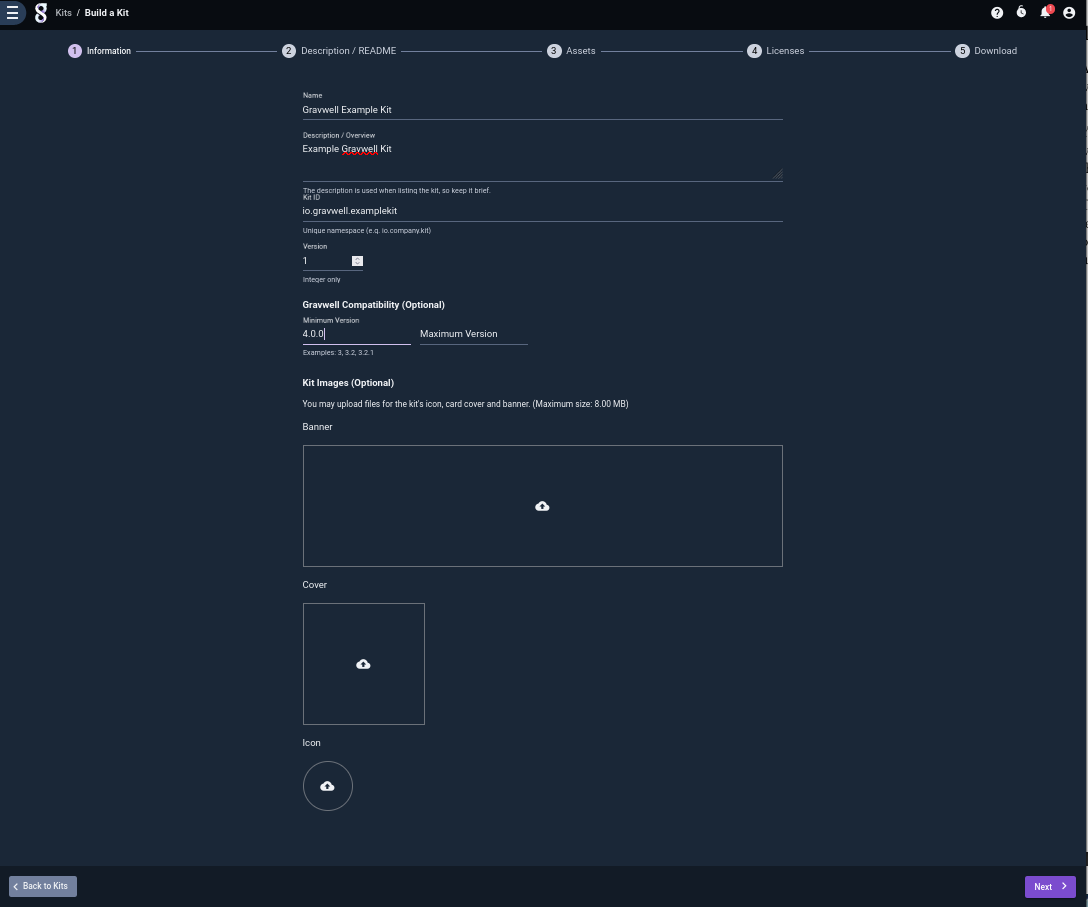
\includegraphics[width=0.8\linewidth]{images/buildwizard1.png}
	\caption{Build wizard, general options}
	\label{fig:buildwizard1}
\end{figure}

The next page (Figure \ref{fig:buildwizard2}) is a markdown editor in which you can write a detailed description of the kit. You can go as simple or as complex as you like, but try to add some detail. 

\begin{figure}[H]
	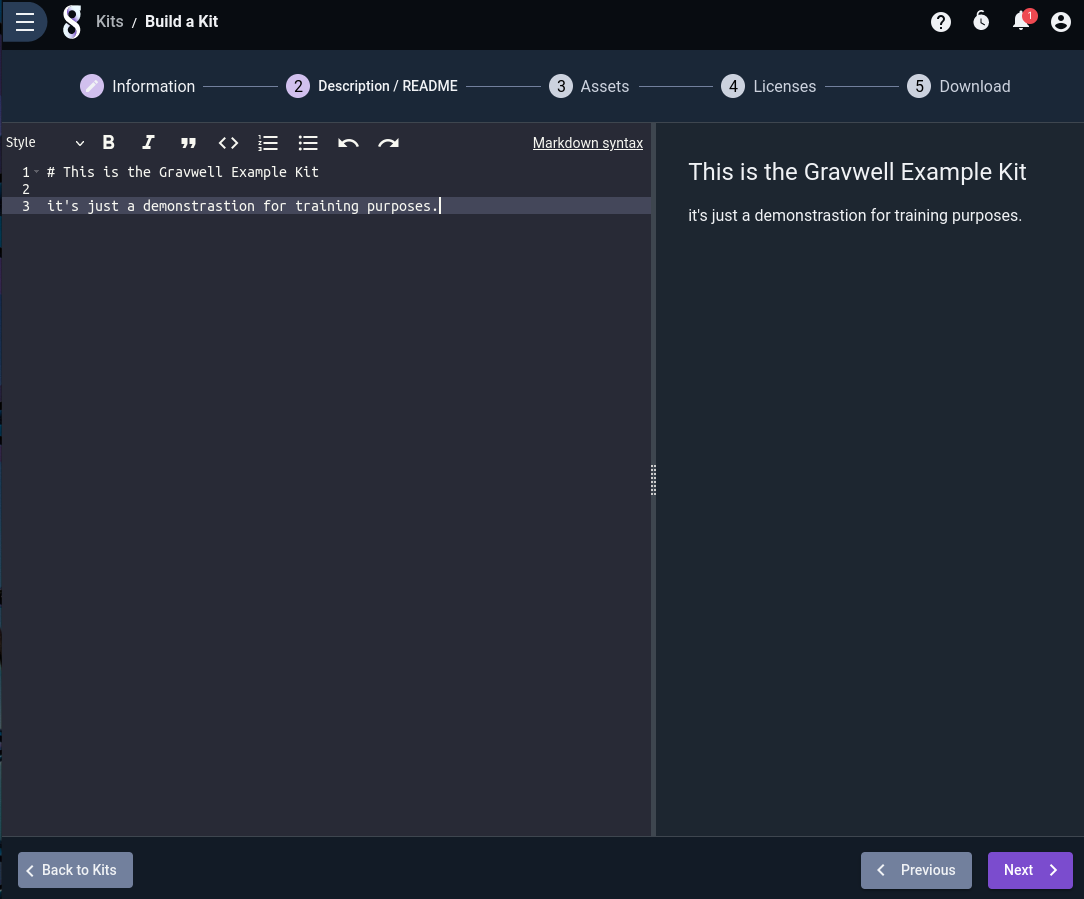
\includegraphics[width=0.8\linewidth]{images/buildwizard2.png}
	\caption{Build wizard, description page}
	\label{fig:buildwizard2}
\end{figure}

The third page, seen in Figure \ref{fig:buildwizard3}, is where you actually select what goes in the kit. You can select an asset category on the left (dashboards, resources, macros, playbooks, etc.), then click to select or deselect items within that category on the right. In the screenshot, we are viewing the Query Library entries and have selected the first 5. We have also previously selected one dashboard.

\begin{figure}[H]
	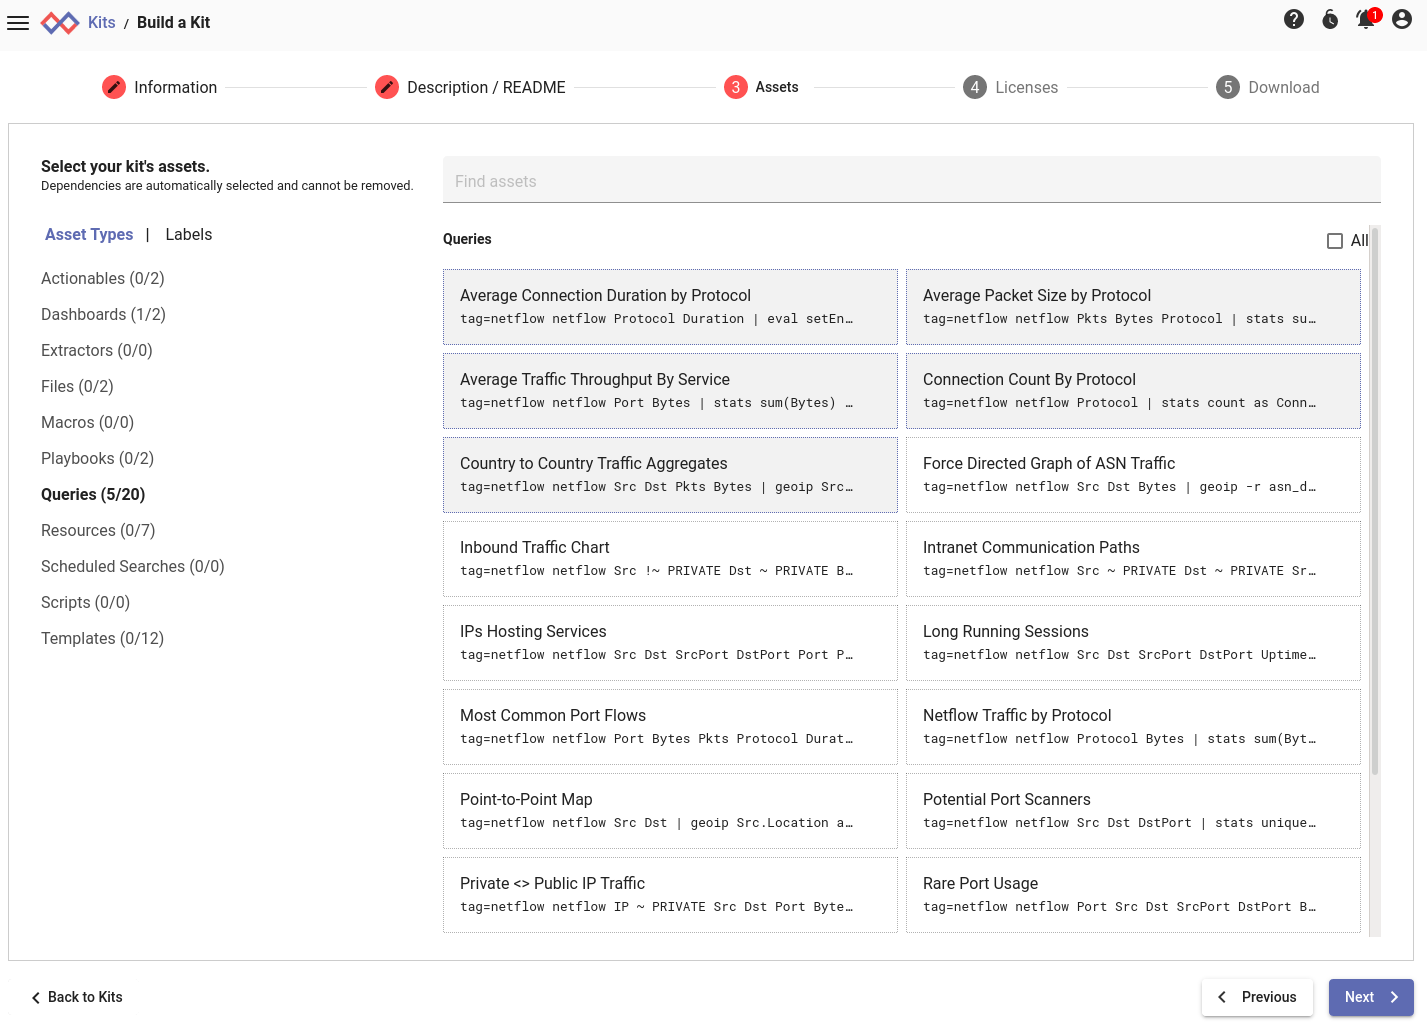
\includegraphics[width=0.8\linewidth]{images/buildwizard3.png}
	\caption{Build wizard, asset selection}
	\label{fig:buildwizard3}
\end{figure}

After selecting assets comes the license page (Figure \ref{fig:buildwizard4}), where you can add licenses if needed--for instance, if you were bundling a third-party resource which requires a license.

\begin{figure}[H]
	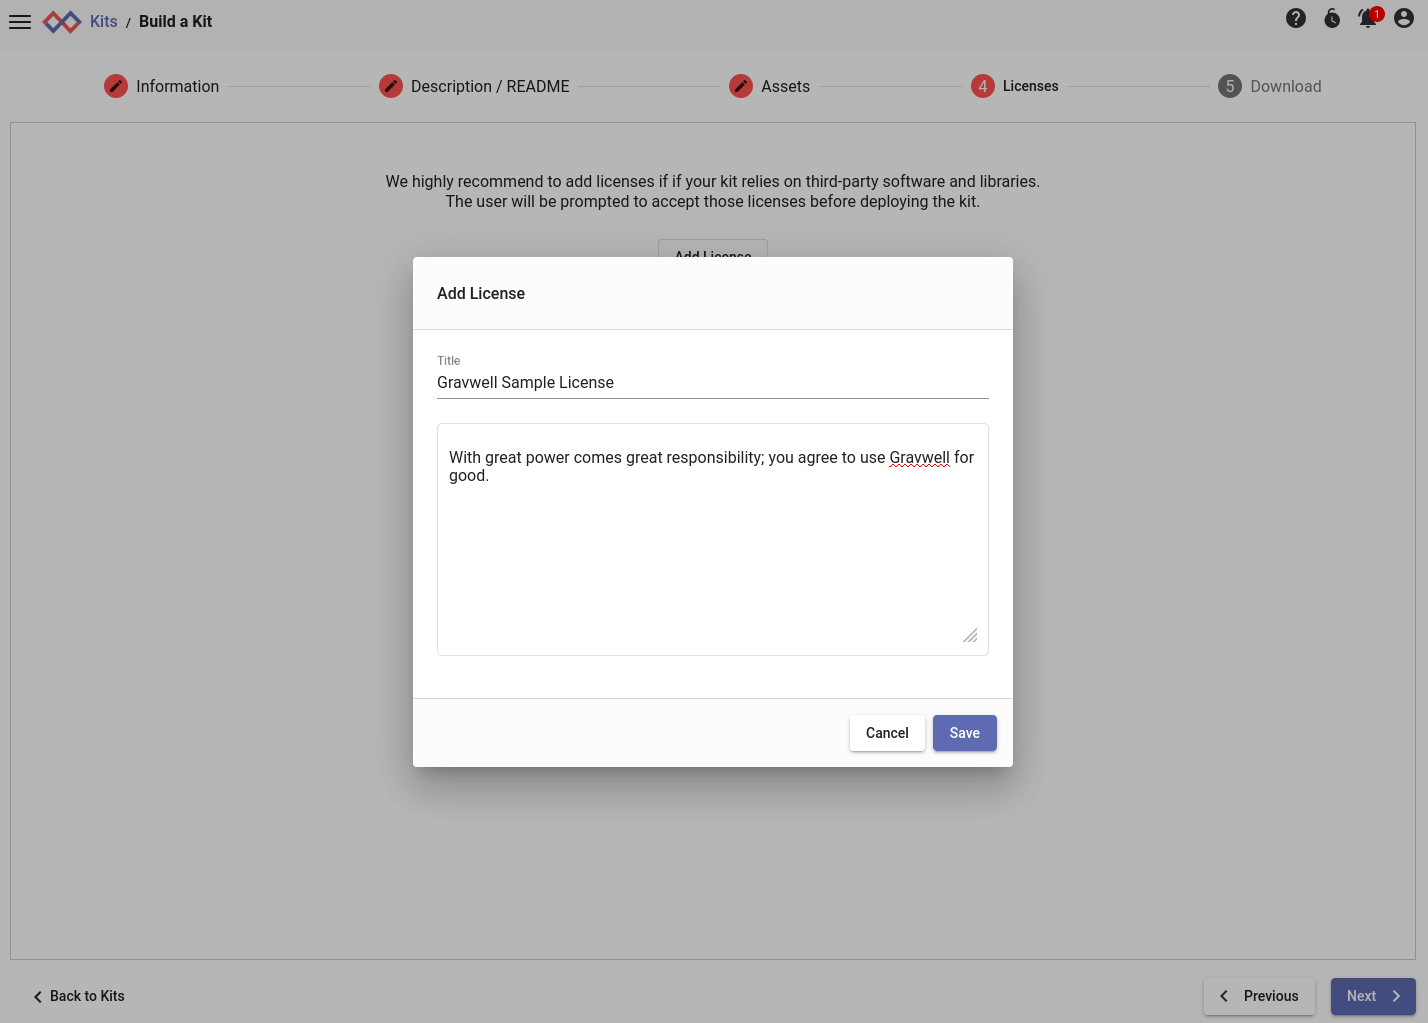
\includegraphics[width=0.8\linewidth]{images/buildwizard4.png}
	\caption{Build wizard, license page}
	\label{fig:buildwizard4}
\end{figure}

After selecting assets, the only step remaining is to download the completed kit. Figure \ref{fig:buildwizard5} shows this page. Note that if you don't click ``Download'', the in-progress kit will not be saved anywhere! You can go back and make changes to any of the previous steps before downloading by clicking the step at the top of the page.

\begin{figure}[H]
	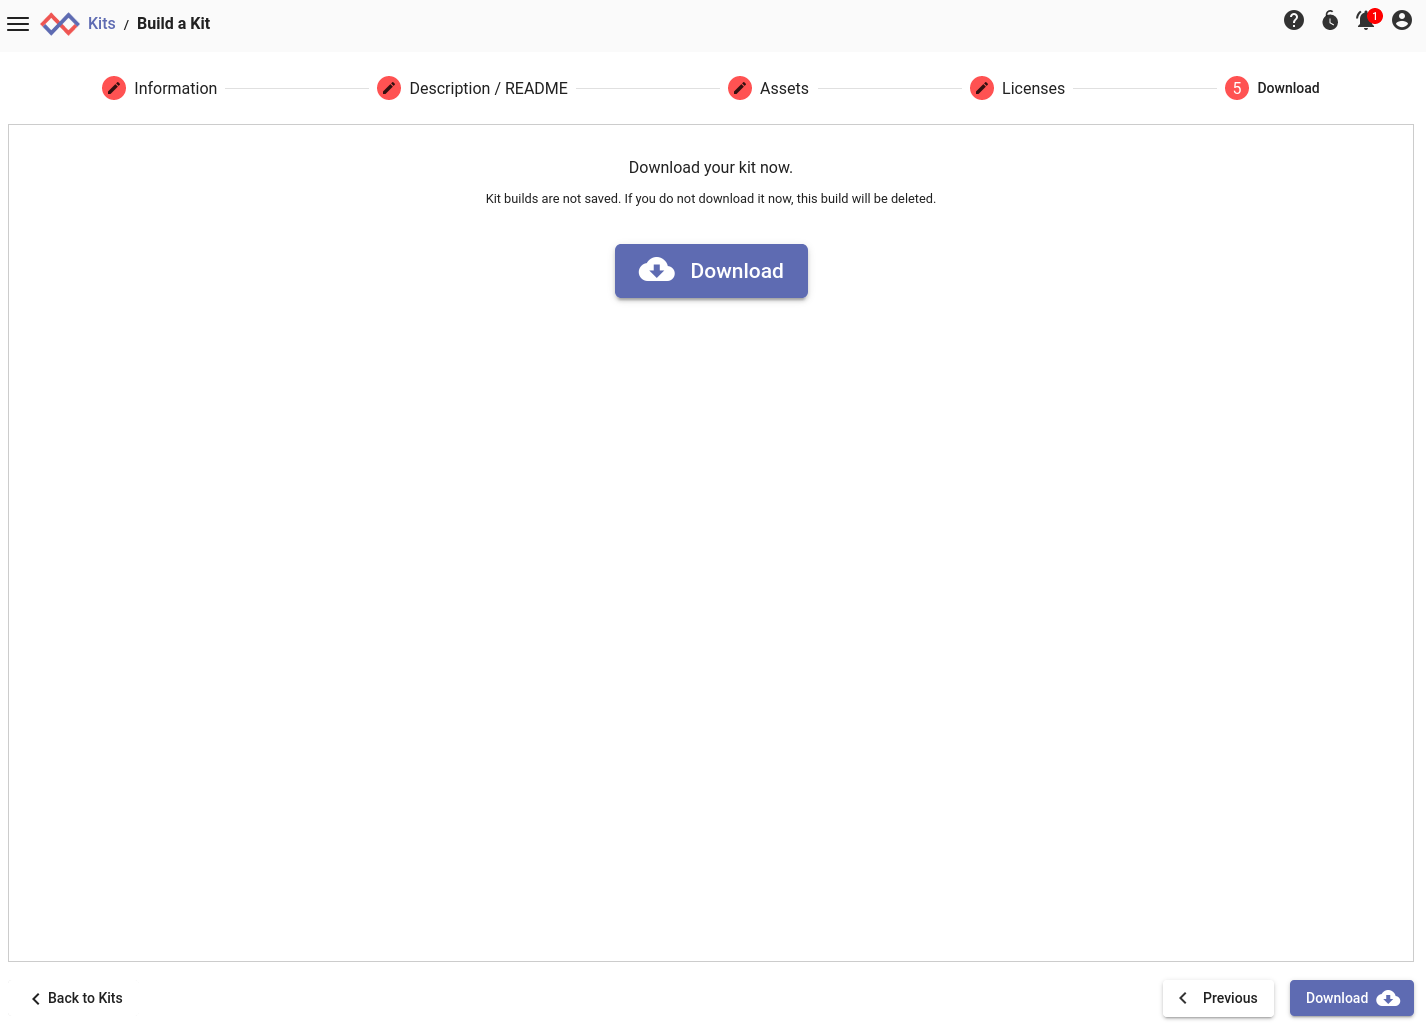
\includegraphics[width=0.8\linewidth]{images/buildwizard5.png}
	\caption{Build wizard download}
	\label{fig:buildwizard5}
\end{figure}
